% Template for PhD theses at the University of Göttingen / GAUSS
% Copyright (C) 2022 Knut Zoch

% This program is free software: you can redistribute it and/or modify
% it under the terms of the GNU General Public License as published by
% the Free Software Foundation, either version 3 of the License, or
% (at your option) any later version.

% This program is distributed in the hope that it will be useful,
% but WITHOUT ANY WARRANTY; without even the implied warranty of
% MERCHANTABILITY or FITNESS FOR A PARTICULAR PURPOSE.  See the
% GNU General Public License for more details.

% You should have received a copy of the GNU General Public License
% along with this program.  If not, see <https://www.gnu.org/licenses/>.

%% Make sure this is processed via pdftex.
\pdfoutput=1

\documentclass[%
               pagenumberstop=false,%   % page numbers at top of page instead
               BCOR=8mm,%               % binding: 0mm (spiral), 6mm (glued)
               ngerman,english,%        % document languages (secondary, main)
               % preliminary=true,%       % activate for timestamp + line numbers
               ]{ktxthss}

\usepackage[%
            % backref=true,%              % create back-references in bibliography
            % eprint=true,%               % show eprint identifiers for all entries
            linking=true,%              % hyperlink journal titles with DOI
            titles=true,%               % show titles of articles (def: true)
            ]{ktxbbltx}

% ==========================================================
% Place any extra packages between this and the following
% horizontal rule, but definitely _not_ afterwards. This
% would screw badly with the hyperref package ...
% ==========================================================

\usepackage{bm}
\usepackage{adjustbox}
\usepackage{multirow}
\usepackage{diagbox}
\usepackage{xfrac}

% Handy packages for creating drafts: create a paragraph of
% random text, and add to-do notes to the document. Probably
% comment them out for the final version.
\usepackage{blindtext}
% \usepackage{todonotes}

% ==========================================================

\usepackage[%
            colorlinks = true,%
            urlcolor   = Venetian,%
            citecolor  = Lime,%
            linkcolor  = Dodger,%
            linktocpage = true,%
            pdfauthor={Your Name},%
            pdftitle={Thesis title},%
            pdfsubject={Thesis subject},%
            pdfkeywords={PhD thesis, dissertation},%
            ]{hyperref}
\usepackage[noabbrev,capitalise]{cleveref}

% Uncomment this line to hide all links in the document
% (cross-references, URLs, bibliography entries). This
% should be used when preparing a print version.
% \hypersetup{hidelinks}

% Adjust these paths to your own needs:
\bibliography{dissertation-bib}
\usepackage{dissertation-defs}

% Choose to include either the English or German cover page +
% back of the title. Adjust thesis title, names etc. in the
% documents "title_[english,german].tex" directly.
% Template for PhD theses at the University of Göttingen / GAUSS
% Copyright (C) 2022 Knut Zoch

% This program is free software: you can redistribute it and/or modify
% it under the terms of the GNU General Public License as published by
% the Free Software Foundation, either version 3 of the License, or
% (at your option) any later version.

% This program is distributed in the hope that it will be useful,
% but WITHOUT ANY WARRANTY; without even the implied warranty of
% MERCHANTABILITY or FITNESS FOR A PARTICULAR PURPOSE.  See the
% GNU General Public License for more details.

% You should have received a copy of the GNU General Public License
% along with this program.  If not, see <https://www.gnu.org/licenses/>.

%%% Title page in English

\newcommand{\HRule}{\rule{\linewidth}{0.5mm}}

\title{%
  \HRule\\[0.4cm]
  \Large
  %% Put the title here. Enforce line breaks with \\.
  Title of the thesis in English\\ Second Line of the Title
  \HRule\\[1.5cm]
}

\subtitle{%
Dissertation\\[1.0cm]
for the award of the degree\\[0.5ex]
%%%%%%%%%%%%%%%%%%%%%%%%%%%%%%%%%%%%%%%%%%%%%%%%%%%%
%%%% In case of the German title 'Dr. rer. nat' %%%%
% ``Doctor rerum naturalium'' (Dr. rer. nat.)\\[0.5ex]
%%%% In case of the international title 'Ph.D.' %%%%
``Doctor of Philosophy'' (Ph.D.)\\[0.5ex]
Division of Mathematics and Natural Sciences\\[0.5ex]
%%%%%%%%%%%%%%%%%%%%%%%%%%%%%%%%%%%%%%%%%%%%%%%%%%%%
of the Georg-August-Universit\"at G\"ottingen\\[1.0cm]
within the Physics doctoral programme\\[0.5ex]
of the Georg-August University School of Science (GAUSS)\\[2.0cm]
}

\author{%
\large
submitted by\\[1.0cm]
\large
Your Name\\[0.5cm]
\large
from Hometown\\[2.0cm]
}

\date{}
\publishers{%
\large
G\"ottingen, 20XX
}

\uppertitleback{% %%% Start of back-of-title-page definition.
\noindent
\underline{Thesis Committee:}\\[0.2cm]
Prof. Dr. X Y\\
{\footnotesize Virtual Institute, Georg-August-Universit\"at G\"ottingen}\\[0.2cm]
Prof. Dr. X Y\\
{\footnotesize Virtual Institute, Georg-August-Universit\"at G\"ottingen}\\[0.2cm]
Prof. Dr. X Y\\
{\footnotesize Virtual Institute, Georg-August-Universit\"at G\"ottingen}\\[0.2cm]

\noindent
\underline{Members of the Examination Board:}\\[0.2cm]
Reviewer: \hspace*{5.2em} Prof. Dr. X Y\\
\hspace*{10.2em}{\footnotesize Virtual Institute, Georg-August-Universit\"at G\"ottingen}\\[0.2cm]
Second Reviewer: \hspace*{1.8em} Priv.-Doz. Dr. X Y\\
\hspace*{10.2em}{\footnotesize Virtual Insitute, Virtual University}\\[0.2cm]
% %%% Only when appointed.
% Additional Reviewer: \hspace*{0.3em} Prof. Dr. X Y\\
% \hspace*{10.2em}{\footnotesize Virtual Institute, Virtual University}\\[0.2cm]

\noindent
\underline{Further members of the Examination Board:}\\[0.2cm]
Prof. Dr. X Y\\
{\footnotesize Virtual Institute, Georg-August-Universit\"at G\"ottingen}\\[0.2cm]
Prof. Dr. X Y\\
{\footnotesize Virtual Institute, Georg-August-Universit\"at G\"ottingen}\\[0.2cm]
Prof. Dr. X Y\\
{\footnotesize Virtual Institute, Georg-August-Universit\"at G\"ottingen}\\[0.2cm]
Prof. Dr. X Y\\
{\footnotesize Virtual Institute, Georg-August-Universit\"at G\"ottingen}\\[1.0cm]

Date of the oral examination: DD Month 20XX \\[1.0cm]

% %%% Only use this when requested.
% \noindent
% Reference: II.Physik-UniG\"o-Diss-20XX/01  %% Not official

}% %%% End of the back-of-title-page definition.
% %
% Title page in German
%

\newcommand{\HRule}{\rule{\linewidth}{0.5mm}}

\title{%
  \HRule\\[0.4cm]
  \Large
  %% Put the title here. Enforce line breaks with \\.
  Titel der Arbeit auf Deutsch\\Zweite Zeile des Titels
  \HRule\\[1.5cm]
}

\subtitle{%
\begin{otherlanguage}{ngerman}
Dissertation\\[1.0cm]
zur Erlangung des mathematisch-naturwissenschaftlichen Doktorgrades\\[0.5ex]
%%%%%%%%%%%%%%%%%%%%%%%%%%%%%%%%%%%%%%%%%%%%%%%%%%%%
%%%% In case of the German title 'Dr. rer. nat' %%%%
\glqq Doctor rerum naturalium\grqq\\[0.5ex]
%%%%%%%%%%%%%%%%%%%%%%%%%%%%%%%%%%%%%%%%%%%%%%%%%%%%
der Georg-August-Universit\"at G\"ottingen\\[1.0cm]
im Promotionsstudiengang Physik\\[0.5ex]
der Georg-August University School of Science (GAUSS)\\[2.0cm]
\end{otherlanguage}
}

\author{%
\large
vorgelegt von\\[1.0cm]
\large
Your Name\\[0.5cm]
\large
aus Hometown\\[2.0cm]
}

\date{}
\publishers{%
\large
G\"ottingen, 2020
}

\uppertitleback{%
\begin{otherlanguage}{ngerman}
\vfill
\noindent
\underline{Betreuungsausschuss:}\\[0.2cm]
Prof. Dr. X Y\\
{\footnotesize Virtual Institute, Georg-August-Universit\"at G\"ottingen}\\[0.2cm]
Prof. Dr. X Y\\
{\footnotesize Virtual Institute, Georg-August-Universit\"at G\"ottingen}\\[0.2cm]
% Prof. Dr. \\
% {\footnotesize Virtual Institute, Georg-August-Universit\"at G\"ottingen}\\[1.0cm]

\noindent
\underline{Mitglieder der Pr\"ufungskommission:}\\[0.2cm]
Referent: \hspace*{1.6em} Prof. Dr. X Y\\
\hspace*{6.2em}{\footnotesize Virtual Institute, Georg-August-Universit\"at G\"ottingen}\\[0.2cm]
Korreferent: \hspace*{0.3em} Priv.-Doz. Dr. X Y\\
\hspace*{6.2em}{\footnotesize Virtual Institute, Virtual University}\\[0.2cm]
% 2. Korreferent: \hspace*{0.3em} Prof. Dr. X Y\\
% \hspace*{10.2em}{\footnotesize Virtual Institute, Virtual University}\\[0.2cm]

\noindent
\underline{Weitere Mitglieder der Pr\"ufungskommission:}\\[0.2cm]
Prof. Dr. X Y\\
{\footnotesize Virtual Institute, Georg-August-Universit\"at G\"ottingen}\\[0.2cm]
Prof. Dr. X Y\\
{\footnotesize Virtual Institute, Georg-August-Universit\"at G\"ottingen}\\[0.2cm]
Prof. Dr. X Y\\
{\footnotesize Virtual Institute, Georg-August-Universit\"at G\"ottingen}\\[0.2cm]
Prof. Dr. X Y\\
{\footnotesize Virtual Institute, Georg-August-Universit\"at G\"ottingen}\\[1.0cm]

Tag der m\"undlichen Pr\"ufung: DD. Month 20XX \\[1.0cm]

% %%% Only use this when requested.
% \noindent
% Reference: II.Physik-UniG\"o-Diss-20XX/01  %% Not official

\end{otherlanguage}
}


% The following command can be used to only generate parts
% of the full document. Put the include paths, as you would
% use it for the \include{tex/file} command, in the the
% following list of files.
% \includeonly{%
  % tex/introduction,
  % tex/results,
  % tex/conclusions,
  % tex/app-add-material,
% }


% ==========================================================
%  B E G I N N I N G   O F   D O C U M E N T
% ==========================================================
\begin{document}

\frontmatter
\pagestyle{empty}
\maketitle

\pagestyle{plain}

% Abstracts in English and German. Choose whatever you consider
% appropriate. My personal thoughts are (assuming the thesis is
% written in English): if the title page is in German, go with
% German and English abstracts (in this order). If the title page
% is English already, the English abstract should follow
% immediately, and the German abstract can be dropped.
% English abstract of the thesis

\begin{center}
  \HRule\\[0.4cm]
  \Large\bfseries
  % Put the thesis title here. Adjust line breaks with the \\
  % command as necessary.
  % ========================================================
  Title of the Thesis in English
  % ========================================================
  \HRule\\[1.5cm]
\end{center}

\begin{center}
  \bfseries
  \large
  Abstract
\end{center}

% Make sure to start the first paragraph with the \noindent
% command to avoid any indentation.
\noindent
First paragraph of the abstract.
\blindtext

Second paragraph of the abstract.
\blindtext

% Make sure to clear a double page before continuing.
\cleardoublepage

% % German abstract of the thesis

\begin{center}
  \HRule\\[0.4cm]
  \Large\bfseries
  % Put the thesis title here. Adjust line breaks with the \\
  % command as necessary.
  % ========================================================
  Titel der Arbeit auf Deutsch
  % ========================================================
  \HRule\\[1.5cm]
\end{center}

\begin{center}
  \bfseries
  \large
  Zusammenfassung
\end{center}

% Only write German text within the following environment.
\begin{otherlanguage}{ngerman}
% Make sure to start the first paragraph with the \noindent
% command to avoid any indentation.
\noindent
Hier das Abstract hin schreiben.
\blindtext

Zweiter Absatz des Abstracts.
\blindtext

\end{otherlanguage}

% Make sure to clear a double page before continuing.
\cleardoublepage


% In case you want to add an epigraph (quote) to the document.
% Settings for the epigraph

\vspace*{\fill}
\setkomafont{dictumtext}{\itshape\small}
\setkomafont{dictumauthor}{\normalfont}
\renewcommand*\dictumwidth{.67\linewidth}
\renewcommand*\dictumauthorformat[1]{--- #1}
\renewcommand*\dictumrule{\vspace*{3ex}}
\dictum{Truth is at variance with our natures, but not so error; and for a very simple reason. Truth requires us to recognise ourselves as limited, but error flatters us with the belief that in one way or another we are subject to no bounds at all.}
\vspace*{6ex}
\dictum[Johann Wolfgang von Goethe (1826)]{Die Wahrheit widerspricht unserer Natur, der Irrtum nicht, und zwar aus einem sehr einfachen Grunde: die Wahrheit fordert, daß wir uns für beschränkt erkennen sollen, der Irrtum schmeichelt uns, wir seien auf ein oder die andere Weise unbegrenzt.}
\vspace*{\fill}


% Make sure to clear a double page before continuing.
\cleardoublepage


\tableofcontents

% In case you want a list of figures, uncomment the following
% line and the index is generated automatically.
% \listoffigures

% In case you want a list of tables, uncomment the following
% line and the index is generated automatically.
% \listoftables

% Either just acknowledgements or maybe a more lengthy preface
% that includes some personal words about the thesis.
% -----------------------------------------------------------
\chapter*{Acknowledgements}
\label{sec:preface}
% -----------------------------------------------------------
% In case this should be added to the table of contents.
% \addcontentsline{toc}{chapter}{Preface}
% \markboth{Preface}{}
% -----------------------------------------------------------

Here you can thank people and acknowledge their help: your supervisor(s), your thesis committee, your examination board, your colleagues, your proofreaders, \dots


% An additional section that lists the exact contributions.
% -----------------------------------------------------------
\chapter*{Contributions by the author}
\label{sec:contributions}
% -----------------------------------------------------------
% In case this should be added to the table of contents.
% \addcontentsline{toc}{chapter}{Contributions}
% \markboth{Preface}{}
% -----------------------------------------------------------

During your PhD you certainly worked on many projects together with other people.
This is a section where you can/should explain what these collaborations looked like.
You might present results in the thesis that include contributions by your collaborators, so this section should be used to clarify what exactly they contributed and on which topics you worked on your own.


% ==========================================================
\mainmatter
\pagestyle{headings}
% ==========================================================

% -----------------------------------------------------------
\chapter{Introduction}
\label{sec:theory}
% -----------------------------------------------------------

Here is space for some general introduction.
The Standard Model (\SM) of elementary particles~%
\cite{Glashow:1961tr,Weinberg:1967tq,Salam:1968rm,Glashow:1970gm,Georgi:1972cj,Gross:1973id,Politzer:1973fx,tHooft:1971akt,tHooft:1971qjg,tHooft:1972tcz,tHooft:1972qbu}
is the best and most complete theory of elementary particles and their interactions to date.
An overview of all particles of the \SM is given in \cref{fig:sm-overview}.

The thesis is organised as follows.
\Cref{chap:results} presents the results, before a summary and conclusions are given in \cref{chap:conclusions}.

\begin{figure}
  \centering
  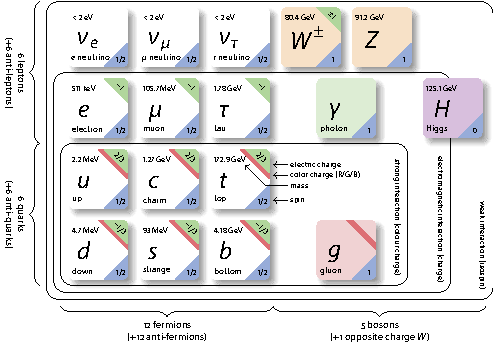
\includegraphics[width=0.86\textwidth]{figures/sm-overview}
  \caption[Particles of the Standard Model]{%
    The particles of the Standard Model.
    The quoted mass values are according to Ref.~\cite{PhysRevD.98.030001}.
    The code for this figure is available on github: \url{https://github.com/knutzk/sm-overview-figure}.
  }
  \label{fig:sm-overview}
\end{figure}


\section{Organisation of this template}

The idea of this template is simple: keep all the different chapters in individual tex files.
That makes the whole writing experience a lot cleaner and it's easier to find stuff.
I would also recommend starting a new line with each sentence, because that makes it easier to track changes in git sentence by sentence.
Tex files for the individual chapters are stored in the \texttt{tex/} subdirectory and then included into the main document with the \texttt{\textbackslash include\{tex/chapter\}} command.
You can use the \texttt{\textbackslash includeonly\{tex/chapter\}} command to switch off some of the chapters of the thesis (without breaking cross-references!).

Figures should go into their own directory, \texttt{figures/}.
And it's probably best to create subdirectories there for each chapter/topic to keep the figures organised in a way.

There are a few extra files to look out for:
%
\begin{itemize}
  \item \texttt{dissertation-defs.sty} -- define abbreviations, common symbols etc. here, and then use them consistently throughout the text. For example, you shouldn't always type \texttt{\$t\textbackslash bar\{t\}\$}, but instead you should pre-define a command such as \texttt{\textbackslash ttbar}. It's gonna make it easier to use these symbols consistently in the text and also makes your latex code much easier to read.
  \item \texttt{dissertation-bib.bib} -- this is where bibliography entries should go. Make sure that all necessary fields are given for each entry type, e.g. an article should always have an author, title, journal, volume, year and pages.
  \item \texttt{tex/abstract\_en/de.tex} -- there are two files for the thesis abstract: one for the English version, one for the German version. Whether you need both is up to you. My personal take is: if the thesis is written in English and the title page is already in English, then there's no need to include a German abstract at all. You should comment/uncomment the abstract files in the main document accordingly.
  \item \texttt{tex/title\_english/german.tex} -- this is where the title page is defined, either in English or in German. Make a choice and comment/uncomment in the main document accordingly.
  \item \texttt{tex/epigraph.tex} -- this is where you could put a quote or some other introductory statement. Comment/uncomment in the main document as you wish.
  \item \texttt{tex/preface.tex} -- this can either be a full-blown preface or just some space to acknowledge other people's help in achieving this manuscript.
  \item \texttt{tex/contributions.tex} -- here you can specify your personal contributions to the projects that you summarise in the thesis. Make sure to discuss this section and what you put there with your supervisor.
\end{itemize}


% Describe the main results

\chapter{Results}
\label{chap:results}

Write the results here.
And we can make a reference to \cref{tab:results-yields}.
\blindtext

We can also add a formula with
%
\begin{align}
  \label{eq:conclusions-xsec}
  \sigma^{\text{fid}} (\ttbar)
  = 291.1 \pm 0.8 \stat ^{+2.9}_{-2.4} \syst \si{\fb}
  = 291.1 \, ^{+3.0}_{-2.5} \; \si{\fb} \, ,
\end{align}
%
corresponding to total relative uncertainties of $^{+\SI{1.0}{\percent}}_{-\SI{0.9}{\percent}}$.


\begin{table}
  \centering
  \caption[Event Yields]{%
    Example of a table showing event yields. 
    The table format is specified in such a way that values are aligned properly.
  }
  \label{tab:results-yields}
  \footnotesize
  \begin{tabular}{%
    l
    S[table-format=3.0] @{${}\pm{}$} S[table-format=2.0]
    S[table-format=3.0] @{${}\pm{}$} S[table-format=2.0]
    S[table-format=4.0] @{${}\pm{}$} S[table-format=2.0]
    S[table-format=4.0] @{${}\pm{}$} S[table-format=3.0]
    }
    \toprule
    & \multicolumn{2}{c}{2015/16} & \multicolumn{2}{c}{2017} & \multicolumn{2}{c}{2018} & \multicolumn{2}{c}{full dataset} \\
    \midrule
    \ttbar & 234 & 12 & 948 & 40 & 947  & 50 & 9371 & 130 \\
    \Wjets & 23  & 3  & 32  & 3  & 74   & 9  & 384  & 15  \\
    \midrule
    Total \MC & 304 & 40 & 978 & 50 & 1027 & 70 & 9836 & 160 \\
    \midrule
    Data & \multicolumn{2}{l}{843} & \multicolumn{2}{l}{987} & \multicolumn{2}{l}{1373} & \multicolumn{2}{l}{3291} \\
    \bottomrule
  \end{tabular}
\end{table}


% Summary and conclusions

\chapter{Summary and conclusions}
\label{chap:conclusions}

Write your conclusiosn here.


% ==========================================================
\printbibliography
% ==========================================================

\appendix


\chapter{Additional material XY}

An appendix with some additional material.


\end{document}
